%!TEX TS-program = xelatex
%!TEX encoding = UTF-8 Unicode

\documentclass[11pt]{extarticle}
% extarticle is like article but can handle 8pt, 9pt, 10pt, 11pt, 12pt, 14pt, 17pt, and 20pt text

\def \ititle {Mindreading and Joint Action}
\def \isubtitle {}
\def \iauthor {Stephen A. Butterfill}
\def \iemail{s.butterfill@warwick.ac.uk}
\date{}

\input{$HOME/Documents/submissions/preamble_steve_handout}


%itemize bullet should be dash
\renewcommand{\labelitemi}{$-$}

\begin{document}

\begin{multicols}{3}

\setlength\footnotesep{1em}

\bibpunct{}{}{,}{s}{}{,}  %use superscript TICS style bib

\bibliographystyle{newapa} %apalike

%\maketitle
%\tableofcontents



\

\begin{center}
{\Large
\textbf{Mindreading \& Joint Action}
}

Heidelberg, 19 May 2011

Stephen A. Butterfill

<s.butterfill@warwick.ac.uk>

\end{center}



\

\begin{center}
{\Large
\textbf{I.\ Minimal Theory of Mind}
}
\end{center}



\section{Abilities vs.\ cognition}

A \emph{theory of mind ability} is an ability that exists in part because exercising it brings benefits obtaining which depends on exploiting or influencing facts about others’ mental states.  

\emph{Theory of mind cognition} paradigmatically involves ascribing propositional attitudes such as beliefs, desires and intentions to give rationalising causal explanations of action. 


\section{Theory of mind abilities are widespread}
Children in their second year use pointing to provide information to others\citep{Liszkowski:2006ec} in ways that reflect their partners’ ignorance or knowledge;\citep{Liszkowski:2008al} provide more information to ignorant than knowledgeable partners when making requests;\citep{ONeill:1996um}  predict actions of agents with false beliefs about the locations of objects;\citep{Onishi:2005hm,Southgate:2007js} and select different ways of helping others depending on whether their beliefs are true or false.\citep{Buttelmann:2009gy}

Scrub-jays selectively re-cache their food in ways that prevent competitors from knowing its location.\citep{Clayton:2007fh}

Chimpanzees select routes to approach food which conceal them from a competitor’s view,\citep{Hare:2006ih} and retrieve food using strategies that optimise their return given what a dominant competitor has seen.\citep{Hare:2001ph}



\section{Theory of mind cognition is hard}
Conceptually demanding:
\begin{itemize}\itemsep0pt
\item Acquisition takes several years\citep{Wimmer:1983dz,Wellman:2001lz}
\item Tied to the development of executive function\citep{Perner:1999yr,Sabbagh:2006ke} and language\citep{Astington2005ot}
\item Development facilitated by explicit training\citep{Slaughter:1996fv} and siblings\citep{Clements:2000nc,Hughes:2004zj}
\end{itemize}
%
Cognitively demanding: 
\begin{itemize}
\item Requires attention and working memory in fully competent adults\citep{Apperly:2008jv,McKinnon:2007rr}
\end{itemize}


\

{\Large
\textbf{First Question}
What could two-year-olds, scrub-jays and chimpanzees represent that would enable them, within limits, to track others’ propositional attitudes?}




\section{How to construct a minimal theory of mind}
An agent’s \emph{field} is a set of objects related to the agent by proximity, orientation, lighting and other factors.

An agent \emph{encounters} an object just if it is in her field.

A \emph{goal-directed action} is a sequence of object-directed actions, which (1) has an outcome that  is an outcome of the whole sequence and not any of its constituents, and (2) occurs in order to bring about this outcome.


\textbf{Principle 1}: one can’t goal-directedly act on an object unless one has encountered it.

Application: subordinate chimps retrieve food when a dominant is not informed of its location.\citep{Hare:2001ph}

Application: when observed scrub-jays prefer to cache in shady, distant and occluded locations.\citep{Dally:2004xf,Clayton:2007fh}

An agent \emph{registers} an object at a location just if she most recently encountered the object at that location.

A registration is \emph{correct} just if the object is at the location it is registered at.

\textbf{Principle 2}: correct registration is a condition of successful action.

Applications: 12-month-olds point to inform depending on their informants’ goals and ignorance;\citep{Liszkowski:2008al} chimps retrieve food when a dominant is misinformed about its location;\citep{Hare:2001ph} scrub-jays observed caching food by a competitor later re-cache in private.\citep{Clayton:2007fh,Emery:2007ze}

 
\textbf{Principle 3}: when an agent performs a goal-directed action and the goal specifies an object, the agent will act as if the object were actually in the location she registers it at.

Applications: false belief tasks \citep{Onishi:2005hm,Southgate:2007js,Buttelmann:2009gy}

\

\

\begin{center}
{\Large
\textbf{II.\ Joint Action}
}
\end{center}




A \emph{joint action} is an event with two or more agents.\citep%[p.\ 366]
{ludwig_collective_2007}

A \emph{goal} is an outcome to which one or more actions are, or might be, directed.  A \emph{goal-state} is an intention or other state of an agent linking an action to a particular goal to which it is directed.

A \emph{goal-directed joint action} is a joint action which, taken as a whole, is directed to a goal.

An outcome is the \emph{teleological function of an action} just if (i) in the past, actions of this type have caused outcomes of this type; (ii) this action happens now in part because (i).


`the unique aspects of human cognition ... were driven by, or even constituted by, social co-operation. ...
[R]egular participation in cooperative, cultural interactions during ontogeny leads children to construct uniquely powerful forms of cognitive representation.'
\citep%[pp.\ 1-3]
{Moll:2007gu}


`perception, action, and cognition are grounded in social interaction
 … functions traditionally considered hallmarks of individual cognition originated through the need to interact with others' \citep%[p.\ 103]
{Knoblich:2006bn}





{\Large
\textbf{Second Question}
Which theory of mind cognition is required for joint action?
}



\section{The standard view: shared intention}

`I take a collective action to involve a collective intention.'  \citep%[p.\ 5]
{Gilbert:2006wr}

`The sine qua non of collaborative action is a joint goal [shared intention] and a joint commitment’ 
\citep%[p.\ 181]
{tomasello:2008origins}

`the key property of joint action lies in its internal component \ldots \ in the participants’ having a ``collective'' or ``shared'' intention.' \citep%[pp. 444-5]
{alonso_shared_2009}

`Shared intentionality is the foundation upon which joint action is built.' \citep%[p.\ 381]
{Carpenter:2009wq}

`it is precisely the meshing and sharing of psychological states \ldots \ that holds the key to understanding how humans have achieved their sophisticated and numerous forms of joint activity'
\citep%[p.\ 369]
{Call:2009fk}



\section{What is shared intention?}

The functional role of shared intentions is to: 
(i) coordinate activities; (ii) coordinate planning; and (iii) provide a framework to structure bargaining.\citep%[p.\ 99]
{Bratman:1993je}

For you and I to have a shared intention that we J it is sufficient that: `(1)(a) I intend that we J and (b) you intend that we J; (2) I intend that we J in accordance with and because of la, lb, and meshing subplans of la and lb; you intend that we J in accordance with and because of la, lb, and meshing subplans of la and lb; (3) 1 and 2 are common knowledge between us'.\citep%[View 4]
{Bratman:1993je}


`each agent does not just intend that the group perform the […] joint action. Rather, each agent intends as well that the group perform this joint action in accordance with subplans (of the intentions in favor of the joint action) that mesh' \citep%[p.\ 332]
{Bratman:1992mi}

`philosophers ... postulate complex intentional structures that often seem to be beyond human cognitive ability in real-time social interactions.'
\citep%[p.\ 2022]
{Knoblich:2008hy}




\

\begin{center}
  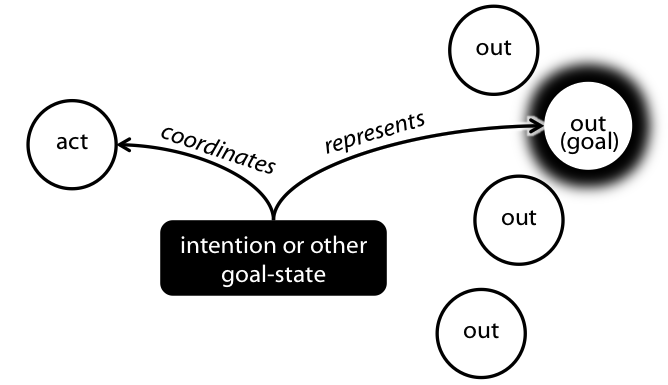
\includegraphics[width=0.3\textwidth]{standard_story.png}
\emph{Figure}: The standard story for individual action.
\end{center}



\section{Goal-directed joint action without shared intention}

\textbf{Distributive goal}.  The \emph{distributive goal} of two or more agents' activities is G: each agent's activities are individually directed to G.

\textbf{Collective goal}.  The \emph{collective goal} of a joint action is G:
(a) each agent’s activities are individually directed to G (i.e. G is a distributive goal);
(b) the agents’ activities are coordinated; and 
(c) coordination of this type would normally  facilitate occurrences of outcomes of G's type

\textbf{Shared goal}.  The \emph{shared goal} of two or more agents' activities is G: (a) G is a collective goal of their activities; 
(b) each agent can identify each of the other agents in a way that doesn't depend on knowledge of the goal or	 actions directed to it;
(c) each agent expects each of the other agents to perform activities directed to G; and 
(d) each agent expects G to occur as a common effect of all their goal-directed actions, or to be partly constituted by all of their goal-directed actions.


\ 

{\Large
\textbf{Third Question}
How might abilities to engage in joint action be involved in the emergence, in evolution or development, of full-blown theory of mind cognition?
}

\textbf{ordinary 3$^{\textrm{\tiny rd}}$ person interpretation}: we determine which outcomes her behaviour is a means of bringing about and then suppose that the goals of her actions are to bring about one or more of these outcomes.

\textbf{the problem of opaque means}: ordinary 3$^{\textrm{\tiny rd}}$ person interpretation may fail when it is not known which outcomes a behaviour is a means of bringing about, especially where a novel tool or communicative device is used.

\textbf{your-goal-is-my-goal}: (1) We are about to engage in some joint action; (2) I am not about to change my goal; therefore (3) The others will each individually perform actions directed to my goal.


`to understand pointing, the subject needs to understand more than the individual goal-directed behaviour. She needs to understand that ... the other attempts to communicate to her ...  and ... the communicative intention behind the gesture'\citep{Moll:2007gu}

`the adult’s social cues conveyed her communicative intent, which in turn encouraged the child to `see through the sign'.'
\citep%[p.\ 118]
{leekam_adults_2010}

\footnotesize 
\bibliography{$HOME/endnote/phd_biblio}

\end{multicols}

\end{document}